%% abtex2-modelo-trabalho-academico.tex, v-1.9.2 laurocesar
%% Copyright 2012-2014 by abnTeX2 group at http://abntex2.googlecode.com/ 
%%
%% This work may be distributed and/or modified under the
%% conditions of the LaTeX Project Public License, either version 1.3
%% of this license or (at your option) any later version.
%% The latest version of this license is in
%%   http://www.latex-project.org/lppl.txt
%% and version 1.3 or later is part of all distributions of LaTeX
%% version 2005/12/01 or later.
%%
%% This work has the LPPL maintenance status `maintained'.
%% 
%% The Current Maintainer of this work is the abnTeX2 team, led
%% by Lauro César Araujo. Further information are available on 
%% http://abntex2.googlecode.com/
%%
%% This work consists of the files abntex2-modelo-trabalho-academico.tex,
%% abntex2-modelo-include-comandos and abntex2-modelo-references.bib
%%

% ------------------------------------------------------------------------
% ------------------------------------------------------------------------
% abnTeX2: Modelo de Trabalho Academico (tese de doutorado, dissertacao de
% mestrado e trabalhos monograficos em geral) em conformidade com 
% ABNT NBR 14724:2011: Informacao e documentacao - Trabalhos academicos -
% Apresentacao
% ------------------------------------------------------------------------
% ------------------------------------------------------------------------

\documentclass[
	% -- opções da classe memoir --
	12pt,				% tamanho da fonte
	openright,			% capítulos começam em pág ímpar (insere página vazia caso preciso)
	twoside,			% para impressão em verso e anverso. Oposto a oneside
	a4paper,			% tamanho do papel. 
	% -- opções da classe abntex2 --
	%chapter=TITLE,		% títulos de capítulos convertidos em letras maiúsculas
	%section=TITLE,		% títulos de seções convertidos em letras maiúsculas
	%subsection=TITLE,	% títulos de subseções convertidos em letras maiúsculas
	%subsubsection=TITLE,% títulos de subsubseções convertidos em letras maiúsculas
	% -- opções do pacote babel --
	%english,			% idioma adicional para hifenização
	brazil
	%french,				% idioma adicional para hifenização
	%spanish,			% idioma adicional para hifenização
	%brazil				% o último idioma é o principal do documento
	%english
	]{abntex2}

% ---
% Pacotes básicos 
% ---
\usepackage{lmodern}			% Usa a fonte Latin Modern			
\usepackage[T1]{fontenc}		% Selecao de codigos de fonte.
\usepackage[utf8]{inputenc}		% Codificacao do documento (conversão automática dos acentos)
\usepackage{lastpage}			% Usado pela Ficha catalográfica
\usepackage{indentfirst}		% Indenta o primeiro parágrafo de cada seção.
\usepackage{color}				% Controle das cores
\usepackage{graphicx}			% Inclusão de gráficos
\usepackage{microtype} 			% para melhorias de justificação
\usepackage{listings} 			% para llistas de codigo
\usepackage{caption} 			% para legendas nas subpictures
\usepackage{subcaption} 			% para legendas nas subpictures
% ---
		
% ---
% Pacotes adicionais, usados apenas no âmbito do Modelo Canônico do abnteX2
% ---
\usepackage{lipsum}				% para geração de dummy text
% ---

% ---
% Pacotes de citações
% ---
\usepackage[brazilian,hyperpageref]{backref}	 % Paginas com as citações na bibl
\usepackage[alf]{abntex2cite}	% Citações padrão ABNT

% --- 
% CONFIGURAÇÕES DE PACOTES
% --- 

% ---
% Configurações do pacote backref
% Usado sem a opção hyperpageref de backref
\renewcommand{\backrefpagesname}{Cited in page(s):~}
% Texto padrão antes do número das páginas
\renewcommand{\backref}{}
% Define os textos da citação
\renewcommand*{\backrefalt}[4]{
	\ifcase #1 %
		No citation in the text.%
	\or
		Cited in page #2.%
	\else
		Cited #1 times in pages #2.%
	\fi}%
% ---

% ---
% Informações de dados para CAPA e FOLHA DE ROSTO
% ---
\titulo{Estágio Supervisionado na RBS TV em 2014/1}
\autor{Lucas Pereira Endres}
\local{Porto Alegre}
\data{2014}
\orientador{Altamiro Amadeu Susin}
%\coorientador{André Borin Soares}
\instituicao{%
  Universidade Federal do Rio Grande do Sul
  \par
  Escola de Engenharia
  \par
  Departamento de Engenharia Elétrica}
%\tipotrabalho{Graduation Thesis}
\tipotrabalho{Relatório de Estágio Supervisionado}
% O preambulo deve conter o tipo do trabalho, o objetivo, 
% o nome da instituição e a área de concentração 
\preambulo{ Estágio em engenharia elétrica na RBS TV Porto Alegre.}
% ---


% ---
% Configurações de aparência do PDF final

% alterando o aspecto da cor azul
\definecolor{blue}{RGB}{41,5,195}

% informações do PDF
\makeatletter
\hypersetup{
     	%pagebackref=true,
		pdftitle={\@title}, 
		pdfauthor={\@author},
    	pdfsubject={\imprimirpreambulo},
	    pdfcreator={LaTeX with abnTeX2},
		pdfkeywords={Multiplexation}{MPEG2}{ISDB-T}{Transport Stream}, 
		colorlinks=true,       		% false: boxed links; true: colored links
    	linkcolor=blue,          	% color of internal links
    	citecolor=blue,        		% color of links to bibliography
    	filecolor=magenta,      		% color of file links
		urlcolor=blue,
		bookmarksdepth=4
}
\makeatother
% --- 

% --- 
% Espaçamentos entre linhas e parágrafos 
% --- 

% O tamanho do parágrafo é dado por:
\setlength{\parindent}{1.3cm}

% Controle do espaçamento entre um parágrafo e outro:
\setlength{\parskip}{0.2cm}  % tente também \onelineskip

% ---
% compila o indice
% ---
\makeindex
% ---

\lstset{
	basicstyle=\footnotesize\ttfamily,
	%framextopmargin=50pt,
	%frame=lrtb
    language=C,
    frame=single,
    tabsize=2,
    showspaces=false,
    showstringspaces=false,
    keywordstyle=\color{blue},
    %morekeywords={QStringList,QDate,QString,QIODevice},
    commentstyle=\color{CadetBlue},
    %caption={Zistenie, či sme v daný deň, už záznam o rýchlosti uložili},
    breaklines=true
	}

% ----
% Início do documento
% ----
\begin{document}

% Retira espaço extra obsoleto entre as frases.
\frenchspacing 

% ----------------------------------------------------------
% ELEMENTOS PRÉ-TEXTUAIS
% ----------------------------------------------------------
% \pretextual

% ---
% Capa
% ---
\imprimircapa
% ---

% ---
% Folha de rosto
% (o * indica que haverá a ficha bibliográfica)
% ---
\imprimirfolhaderosto*
% ---

% ---
% RESUMOS
% ---

% resumo em português
\setlength{\absparsep}{18pt} % ajusta o espaçamento dos parágrafos do resumo
\begin{resumo}[Resumo]
 \begin{otherlanguage*}{brazil}
	
%Estudos para a implantação da TV digital no Brasil definiram que o sistema de transmissão deve ser derivado do padrão japonês ISDB-T. Um dos objetivos das organizações públicas ao escolher o padrão japonês era o de permitir um desenvolvimento mais significativo da tecnologia nacional, de modo que a tecnologia japonesa modificada permitiu que centros de pesquisa brasileiros participassem no desenvolvimento da televisão digital. O principal objetivo deste trabalho é desenvolver uma ferramenta que cria um Transport Stream compatível com o padrão brasileiro definido na ABNT NBR15603-1, baseada na norma ISO/IEC13818. Para atingir o objetivo, uma considerável pesquisa foi feita para entender os conceitos fundamentais introduzidos pela ISO/IEC13818, e as diferenças entre a ISO/IEC13818 e a ABNT NBR15603-1. Algumas ferramentas existentes criam fluxos compatíveis com a norma internacional, mas não atendem às modificações brasileiras. Sugere-se portanto uma modificação de uma solução existente, FFmpeg, que agora passa a incluir as estruturas obrigatórias do SBTVD nos fluxos de transporte gerados.

A televisão é o meio de comunicação mais importante no Brasil. No início da última década, decidiu-se digitalizar o sistema de transmissão de TV brasileira. Uma ação do governo unindo pesquisadores de todo o país realizou um estudo sobre vários temas de TV Digital. Codificação de vídeo e áudio, bem como os subsistemas de interatividade, multiplexação, modulação e transmissão estão entre os aspectos estudados do sistema DTV. Como resultado surgiu o SBTVD, o padrão de TV digital brasileiro, que é baseado no padrão japonês de transmissão ISDB-T, e adota os padrões H.264 e HE-AAC para codificação de vídeo e áudio. Hoje em dia, quase todos os países sul-americanos e alguns africanos adotaram o SBTVD. Há grande interesse em ampliara a cobertura TV digital para o interior do país, e é por isso que se ...

O principal objetivo deste trabalho é desenvolver uma ferramenta que cria um Transport Stream compatível com a norma brasileira ABNT NBR15603, que é baseada na norma ISO/IEC 13818-1. Para alcançar este objetivo, realizou-se extensa pesquisa para compreender os conceitos fundamentais introduzidos pela ISO/IEC13818-1 e as diferenças entre esta e a ABNT NBR15603. Algumas ferramentas existentes geram um Transport Stream compatível com as normas internacionais, mas não conseguem obedecer às especificidades brasileiras. Assim, propõe-se uma versão modificada do aplicativo FFmpeg que agora inclui as estruturas obrigatórias do SBTVD no Transport Stream.

 \textbf{Palavras-chaves}: Multiplexação. MPEG2. Transport Stream. SBTVD.
 \end{otherlanguage*}
\end{resumo}

% resumo em inglês
% \begin{resumo}[Abstract]

Studies for the implementation of digital TV in Brazil have identified that the transmission system should be derived from the Japanese standard, ISDB-T. One of the goals of public organizations by choosing the Japanese standard was to allow a more significant development of national technology. Thus, the choice for the modified Japanese technology has allowed Brazilian research centres to participate on the development of digital television. The main objective of this project is develop a tool that creates a Transport Stream which is compliant to the Brazilian standard ABNT NBR15603 which is based in the ISO/IEC 13818-1 standard. To achieve the objective, considerable research was carried out to understand the fundamental concepts introduced by ISO/IEC13818and the differences between ISO/IEC13818-1 and ABNT NBR15603. Some existing tools generate streams compliant to the international standard but not to the Brazilian modifications. A modification is therefore proposed to an existing solution, FFmpeg, which now includes the mandatory structures of SBTVD in generated Transport Streams.

% Television is the most important communication media in Brazil. At the beginning of the last decade, it was decided to digitize the Brazilian TV broadcast system. A government action joining researchers of all around the country carried out a study on several topics of Digital TV. Video and audio coding, along with interactivity and multiplexing, modulation and transmission subsystems are among the studied aspects of the DTV System. What came out is the SBTVD, the Brazilian DTV standard, which is based on the Japanese ISDB-T transmission standard, and adopts H.264 and HE-AAC as video and audio coding standards. Nowadays, almost all South American and some African countries adopted the SBTVD. The main objective of this work is to develop a tool that creates a Transport Stream compliant to the Brazilian standard ABNT NBR15603 which is based on the ISO/IEC 13818-1 standard. To achieve this objective, considerable research was carried out to understand the fundamental concepts introduced by ISO/IEC13818-1 and the differences between this standard and the ABNT NBR15603. Some existing tools generate streams compliant to the international standards but fail to obey the Brazilian specificities. An updated version of the FFmpeg framework is therefore proposed which now includes the mandatory structures of SBTVD in the Transport Stream.

   % \vspace{\onelineskip}
 
   % \noindent 
   % \textbf{Key-words}: Multiplexing. MPEG2. Transport Stream. SBTVD.
 
% \end{resumo}

%% ---
% inserir lista de ilustrações
% ---
\pdfbookmark[0]{\listfigurename}{lof}
\listoffigures*
\cleardoublepage
% ---

% ---
% inserir lista de tabelas
% ---
\pdfbookmark[0]{\listtablename}{lot}
\listoftables*
\cleardoublepage
% ---

% ---
% inserir lista de abreviaturas e siglas
% ---
%\begin{siglas}
%  \item[ABNT] Associação Brasileira de Normas Técnicas
%  \item[ISO] International Standards Organization
%  \item[ARIB]
%  \item[MPEG] Motion Pictures Experts Group ???
%  \item[EBC] Empresa Brasileira de Comunicação
%  \item[]
%  \item[]
%  \item[]
%\end{siglas}

\begin{siglas}
  \item[64QAM] Quadrature Amplitude Modulation with 64 Symbols
  \item[AAC] Advanced Audio Coding
  \item[AAC-LC] Advanced Audio Coding - Low Complexity
  \item[ABNT] Associação Brasileira de Normas Técnicas
  \item[AF] Adaptation Field
  \item[ARIB] Association of Radio Industries and Businesses
  \item[CAT] Conditional Access Table
  \item[CBR] Constant Bit Rate
  \item[CRC] Cyclic Redundancy Check
  \item[DCT] Discrete Cosine Transform
  \item[DTS] Decoding Time Stamp
  \item[DTV] Digital Television
  \item[DVB] Digital Video Broadcasting
  \item[EBC] Empresa Brasileira de Comunicação
  \item[EIT] Event Information Table
  \item[EPG] Electronic Program Guide
  \item[ES] Elementary Stream
  \item[fps] frames per second
  \item[HE-AAC] High-Efficiency Advanced Audio Coding
  \item[HDTV] High Definition TV
  \item[ISDB-T] Integrated Services Digital Broadcasting - Terrestrial
  \item[IEC] International Electrotechnical Commission
  \item[ISO] International Standards Organization
  \item[ITU] International Telegraph Union
  \item[ITU-T] ITU Telecommunication Standardization Sector
  \item[LATM] Low Overhead Audio Transport Multiplex
  \item[LTE] Long Term Evolution
  \item[MPEG] Moving Picture Experts Group
  \item[NIT] Network Information Table
  \item[PAT] Program Association Table
  \item[PCI] Peripheral Component Interconnect
  \item[PCR] Program Clock Reference
  \item[PMT] Program Map Table
  \item[PTS] Presentation Time Stamp
  \item[PES] Packetized Elementary Stream
  \item[PID] Packet ID
  \item[PLL] Phase Locked Loop
  \item[PS] Parametric Stereo
  \item[PS] Program Stream
  \item[PSI] Program Specific Information
  \item[QPSK] Quadrature Phase-Shift Keying
  \item[SBR] Spectral Band Replication
  \item[SBTVD] Sistema Brasileiro de Televisão Digital
  \item[SDT] Service Description Table
  \item[SDTV] Standard Definition TV
  \item[SI] System Information
  \item[STC] System Time Clock
  \item[TOT] Time Offset Table
  \item[TS] Transport Stream
  \item[UHF] Ultra High Frequency
  \item[VBR] Variable Bit Rate
  \item[VCO] Voltage Controlled Oscillator
  \item[]
  \item[]
  \item[]
  
  
\end{siglas}

% ---

% ---
% inserir lista de símbolos
% ---
% \begin{simbolos}
  % \item[\texttt{0xN}] Is the hexadecimal number 'N'
  % \item[DIV] Integer division with truncation of the result towards $-\infty$
  % \item[\%] Modulus operator. Defined only for positive numbers.
  % \item[\texttt{N d}] Is the decimal number 'N'.
 \item[$ \in $] Pertence
% \end{simbolos}
% ---

% ---
% inserir o sumario
% ---
\pdfbookmark[0]{\contentsname}{toc}
\tableofcontents*
\cleardoublepage
% ---



% ----------------------------------------------------------
% ELEMENTOS TEXTUAIS
% ----------------------------------------------------------
\textual

% ----------------------------------------------------------
% Introdução (exemplo de capítulo sem numeração, mas presente no Sumário)
% ----------------------------------------------------------
\chapter[Introduction]{Introduction}
%\addcontentsline{toc}{chapter}{Introduction}
% ----------------------------------------------------------

%Historicamente, a televisão está presente nas casas da maioria dos cidadãos brasileiros e é a principal fonte de
%entretenimento e informação para a população. Nos últimos 10 anos, os novos meios de comunicação digital, tais
%como o computador e o telefone celular, estão sendo adotados pela população de diferentes classes sociais. Um
%dado recente \cite{pnad2011} afirma que, em 2011, 69\% da população brasileira dispunha de uma linha de 
%telefone celular. Embora seja significativa, a participação deste meio ainda é muito inferior à da televisão,
%cuja área de cobertura de sinal atinge 100\% do território por via satelital \cite{starone}, e próximo de
%70\% da população por via terrestre. A televisão é, portanto, o principal canal de comunicação disponível ao 
%grande público no Brasil.

%Ainda que tenha cobertura incomparável às demais tecnologias, a televisão é, a grosso modo, um meio de comunicação
%unidirecional. Não é viável, no sistema de transmissão analógica, haver interatividade dos
%telespectadores com o conteúdo apresentado pela geradora. Se comparada à \textit{Internet}, por exemplo, a televisão
%está em desvantagem nesse aspecto. É possível, no entanto, dotar a programação de interatividade se houver um meio de
%retornar dados para a geradora. Com a interatividade, ao usuário podem ser apresentadas opções de programação e, 
%a partir de sua escolha, o televisor exibe o conteúdo. Assim, se poderia aliar a interatividade da \textit{Internet}
%à abrangência da televisão e com isso promover a inclusão social de regiões remotas, sem acesso à infraestrutura 
%de dados em alta velocidade presente nas grandes metrópoles. Essa tecnologia é inviável com a infraestrutura atual
%da televisão analógica: é impossível enviar através de um único canal analógico mais de um conteúdo de vídeo ou
%áudio simultaneamente.
%
%Como solução a essa dificuldade, desenvolveu-se o sistema de transmissão digital descrito pela norma ISO/IEC 13818, comercialmente conhecido pela sigla que dá nome ao comitê formado para redigí-la, o MPEG2. A norma descreve um padrão de codificação e transmissão de vídeo, áudio e dados e que permite, dentre outras funções, transmitir conteúdos audiovisuais independentes simultaneamente, permitindo assim que o usuário do sistema escolha, dentre as informações enviadas pela geradora, qual ele deseja receber.
%
%Desde 1994, empresas privadas e poder público financiaram pesquisas e testes técnicos para comparar o desempenho de três sistemas de televisão digital que na época eram sabidamente eficientes em seus países de origem: o ATSC, desenvolvido nos Estados Unidos; o DVB, desenvolvido pelos países europeus; e o ISDB, desenvolvido no Japão. Os três sistemas têm diferenças no que tange a codificação do vídeo e do áudio, mas o ISDB e o DVB, por exemplo, compartilham a infraestrutura de transporte de dados do padrão MPEG2, mas diferem nos esquemas de modulação do sinal. Após as avaliações, foi concluído que o sistema com a provável melhor performance no território brasileiro seria baseado no ISDB, japonês, com modificações.
%
%As diferenças entre o padrão ISDB original e o adotado no Brasil referem-se principalmente à codificação de vídeo e à plataforma de interatividade. Com o intuito de promover o desenvolvimento da indústria nacional, o governo determinou a adoção de uma plataforma de interatividade de código aberto, desenvolvida majoritariamente com tecnologia da PUC-RJ, o Ginga. Através desta ferramenta, é possível, por exemplo, levar informações de utilidade pública à população de baixa renda, sem acesso
%à \textit{Internet}, como demonstrou a Caixa Econômica Federal em 2010\cite{caixa}. Contudo, a similaridade do sistema de transmissão brasileiro com o padrão internacional MPEG2 e a não obrigatoriedade da utilização de interfaces interativas até 2015 levou ao desinteresse das geradoras no desenvolvimento da tecnologia,
%de modo que atualmente muito pouco se investe para a criação de equipamentos interativos para a televisão digital em terrítório brasileiro.

Historically, television is present in the homes of most Brazilian citizens and it is the main source of entertainment and information to the population. Over the past 10 years, new digital media such as computer and cell phones are being adopted by the population of different social classes. A recent report \cite{pnad2011} says that in 2011, 69 \% of the population had a mobile phone line. Although significant, the participation of this medium is still far below the television, whose coverage area reaches 100 \% of the territory via satellite \cite{StarOne}, and around 98\% of the population by land \cite{globo}. Television is therefore the main channel of communication available to the general public in Brazil.

Although it has unparalleled coverage to other technologies, television is a mean of unidirectional communication. It is not possible, using the analog TV transmission system, to hand to the viewer interactivity with the content submitted by the broadcaster. Compared to \textit{Internet}, for example, television is at disadvantage in this aspect. It is possible, however, to provide interactive programming if there is a way to return data to the broadcaster. With interactivity, it can be presented to the user program options, and from the user's choice, the TV displays the chosen content. Thus, one could combine the interactivity of \textit{Internet} to television coverage and thereby promote the social inclusion of remote areas without access to infrastructure of high-speed data links, available in the larger cities . This technology is not feasible with the current analog television infrastructure: it is impossible to transmit via a single analog channel more than one video and two audio streams simultaneously.

As a solution to this difficulty, ISO/IEC developed the digital transmission system described by ISO/IEC13818 standard, commercially known by the acronym which names the committee formed to draft it, MPEG2. The specification describes standards of encoding and transmitting video, audio and system data. One key feature for television applications is that it is possible to broadcast multiple audiovisual programs simultaneously, thus allowing the user to select which information he wants to receive among several services sent by one single broadcaster, in the same physical channel.

In Brazil, since 1994, private companies and government funded research and technical tests to compare the performance of three digital television systems that were known to be efficient in their countries of origin at that time: ATSC \cite{ATSC}, developed in the United States; DVB-T \cite{DVB}, developed by a consortium of companies for use in European countries; and ISDB , developed in Japan by ARIB\cite{ARIB}. The three systems have similarities and differences regarding the encoding of video and audio: for example, both the DVB and ISDB use the transport infrastructure of MPEG2 standard, but differ in the modulation schemes. After the evaluations, it was determined that the system with the best performance for Brazilian territory would be based on the Japanese ISDB with some modifications, such as pointed in \cite{decreto8061}.

The differences between the original ISDB and the modified standard used in Brazil mainly relate to video encoding and interactivity platform. In order to promote the development of national industry, the government decided to adopt an open source interactive platform, developed with Ginga, a technology developed mainly by Brazilian researchers\cite{PUCRJ}. Through this tool the broadcaster can, for example, deliver useful information to the low-income population without access to the \textit{Internet}, as an application sugested by one Brazilian Bank in 2010 \cite{caixa}. Another application is a project recently developed by the brazilian public comunication company (EBC), called "Brasil 4D" \cite{consultas}. The users can make appointments with doctors or schedule meetings to solve social security issues, or yet check job offers in real time, all this through the TV remote control. However, the similarity of the Brazilian system with the international standard and the fact that interactive interfaces will not be mandatory until 2015 led to the lack of interest of many broadcasters in the development of applications, so that currently very little is invested in the creation of interactive digital television in Brazilian territory.

A digital television system is composed basically by the group of equipments presented in \autoref{fig:diagrama_blocos_tvd}. At the beginning of the signal flow, there are the video and audio capturing elements, such as cameras and microphones, and the raw signal may be analog or digital depending on the capture technology used. Once captured, the video and audio are compressed and coded through corresponding encoders. The output of the encoders are standardized bitstreams called Elementary Streams. Once the elementary streams leave the encoders, they enter the multiplexer, where all the streams are packetized and embedded into one single stream, which is the main objective of the MPEG2 systems layer. What follows is one key process for the system robustness: the stream is protected with the use of error correction codes to resist to the noisy, multipath channel between the broadcaster and the receiver. Finally, a digital modulation is applied and the modulated stream is sent to the antenna.
 
 \begin{figure}[!h]
\centering
\caption{Block diagram showing digital television basic signal flow.}
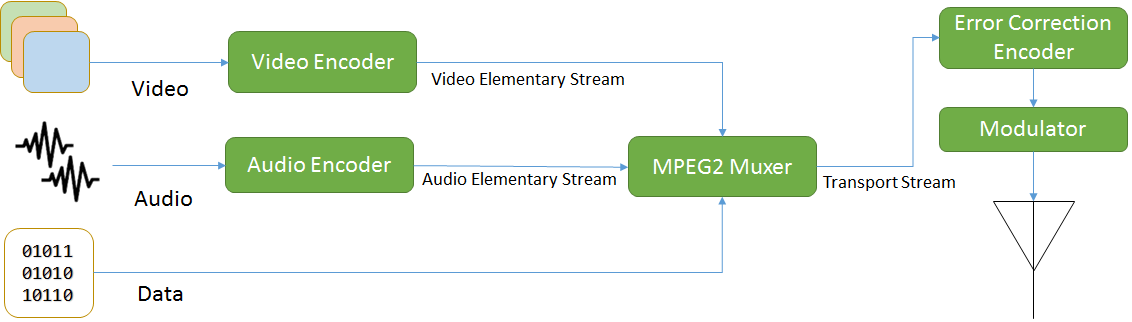
\includegraphics[width=1\linewidth]{figuras/diagrama_blocos_tvd.png}
\label{fig:diagrama_blocos_tvd}
\end{figure}
 
The main difference between analog and digital TV broadcasting systems, at the modulation level, is that in analog TV the multiplexing is in frequency domain, the video signal is sent in a frequency band within the channel bandwidth and the audio in another frequency band. In digital technology, this multiplexing happens in time domain: the multiplexer output has constant bitrate, and for fractions of second only one packet from one of the media sources is sent to the transmitter. In the other side of the channel, the receiver is conceived in such a way that after passing the error correction layer, a \textit{demultiplexer} takes the compound stream and splits it back into elementary bitstreams. They are then sent to the decoders and to audiovisual output devices.

It would be certainly disturbing to the viewer to watch delayed video or audio outputs, thus one challenge of this multiplexing scheme is to synchronize the reproduction of all the streams. To ensure this, presentation time stamps are added periodically into the streams so they can be reproduced in sync.

%O sistema de transmissão de televisão digital funciona, basicamente, coordenando a entrada de fluxos elementares de vídeo, áudio e dados no fluxo de transmissão. Na televisão analógica, a multiplexação é frequencial, ou seja, o sinal de vídeo é enviado em um intervalo de frequências dentro do canal e o sinal de áudio em outro intervalo. Na tecnologia digital, essa multiplexação é feita no tempo: por frações de segundo, apenas um dos sinais é enviado no canal e o receptor armazena os sinais independentemente para depois fazer a decodificação. No momento da reprodução dos sinais, é preciso que haja sincronismo nos fluxos de vídeo e áudio.

The Presitential Act number 8061\cite{decreto8061}, from july 29, 2013, establishes the chronogram of analog brodcasts shutdown. Until december 31, 2018, all analog transmitters shall be deactivated and the channels shall be vacated. The radio-frequency grants will then be returned to the government, that plans to use the 700MHz band to the 4G mobile telephone service, LTE.

%O Decreto presidencial número 8061, de 29 de julho de 2013, estabelece o cronograma de desligamento dos sistemas de transmissão de televisão analógica. Até 31 de dezembro de 2018, todos os transmissores analógicos devem ser desativados e os canais de radiofrequência devolvidos à união... COLOCAR REFERENCIA! 

The objective of this project is to develop a simple, yet flexible, tool to handle the Systems layer on SBTVD standard. Basically, by using this tool one is able to produce a SBTVD-compatible binary file containing a Transport Stream that can be used to broadcast recorded video and audio streams into appropriate receivers. Many commercial solutions for this objective are available on the market, so the target here was not to develop a consumer product, but rather something more academic, educational, where most of the configurations can be modified as desired. The main UFRGS internal client is the SBTVD set top box project, which is developing a set-top-box in as a System on Chip architecture in FPGA. In order to run tests of the entire system, streams with different multiplexing setups must be broadcast. When received, the way that the decoder handles them must be analysed.

The project workflow was the following. The first step was to study the ABNT NBR15603 standard and the references in it to the ISO/IEC 13818 standard and to the ARIB STD-B10 standard. Here the target was to understand how the Systems Layer should work and identify which parts were mandatory and optional. While discussing the project at the very first weeks, it was decided to evaluate the possibility of develop the tool from scratch. This was before the first step was accomplished, because other people in the lab had already done some research and had concluded that the available freeware tools couldn't handle the SBTVD characteristics. During the author's own research on the Internet, some interesting tools were identified, and instead of developing from scratch, it seemed by then more reasonable to profit of an existent framework.

Once it was decided that an existing tool would be modified, the third step was to add the missing features in order to make it compatible with the SBTVD, and finally the features were tested on several receivers. The practical objective of the project is to provide a tool that creates Transport Streams with three key features: synchronous audiovisual presentation, compliance to the SBTVD standard and multiple services. Eventually, if any mandatory structures are only informational and do not block the system from working, they might be left for further development.

%In the first few weeks, no freeware solution had been found to meet these requirements, so it was proposed that the tool should be developed from scratch. After extra research efforts, some existing open source applications were found and fortunately they already met some of the requirements, but all were developed respecting the pure MPEG2 standard and naturally didn't include some of the brazilian system requirements. It was then proposed that the project target was to deliver no longer a solution from scratch, bu rather something based on one of the existing tools, adapting it to comprise the brazilian standard requirements. A discussion on the analysed tools is presented in the following chapters.

% The project objective is to develop an academic solution  not develop a customer solution, but rather an academic solution, in which one may broadcast streams without the restrictions of a commercial solution, although one may integrate the software to a modulator PCI board and a amplifier to constitute a small, cheap TV Station.

%In \autoref{codecs}, a brief description of the encoders chosen to integrate the standard is presented. In \autoref{}, 

%% FIM DA INTRODUÇÃO ESCRITA PARA O TCC

% ----------------------------------------------------------
% PARTE
% ----------------------------------------------------------
%\part{Preparação da pesquisa}
% ----------------------------------------------------------

% ---
% Capitulo com exemplos de comandos inseridos de arquivo externo 
% ---
%%% abtex2-modelo-include-comandos.tex, v-1.9.2 laurocesar
%% Copyright 2012-2014 by abnTeX2 group at http://abntex2.googlecode.com/ 
%%
%% This work may be distributed and/or modified under the
%% conditions of the LaTeX Project Public License, either version 1.3
%% of this license or (at your option) any later version.
%% The latest version of this license is in
%%   http://www.latex-project.org/lppl.txt
%% and version 1.3 or later is part of all distributions of LaTeX
%% version 2005/12/01 or later.
%%
%% This work has the LPPL maintenance status `maintained'.
%% 
%% The Current Maintainer of this work is the abnTeX2 team, led
%% by Lauro César Araujo. Further information are available on 
%% http://abntex2.googlecode.com/
%%
%% This work consists of the files abntex2-modelo-include-comandos.tex
%% and abntex2-modelo-img-marca.pdf
%%

% ---
% Este capítulo, utilizado por diferentes exemplos do abnTeX2, ilustra o uso de
% comandos do abnTeX2 e de LaTeX.
% ---
 
\chapter{Resultados de comandos}\label{cap_exemplos}

\chapterprecis{Isto é uma sinopse de capítulo. A ABNT não traz nenhuma
normatização a respeito desse tipo de resumo, que é mais comum em romances 
e livros técnicos.}\index{sinopse de capítulo}

% ---
\section{Codificação dos arquivos: UTF8}
% ---

A codificação de todos os arquivos do \abnTeX\ é \texttt{UTF8}. É necessário que
você utilize a mesma codificação nos documentos que escrever, inclusive nos
arquivos de base bibliográficas |.bib|.

% ---
\section{Citações diretas}
\label{sec-citacao}
% ---

\index{citações!diretas}Utilize o ambiente \texttt{citacao} para incluir
citações diretas com mais de três linhas:

\begin{citacao}
As citações diretas, no texto, com mais de três linhas, devem ser
destacadas com recuo de 4 cm da margem esquerda, com letra menor que a do texto
utilizado e sem as aspas. No caso de documentos datilografados, deve-se
observar apenas o recuo \cite[5.3]{NBR10520:2002}.
\end{citacao}

Use o ambiente assim:

\begin{verbatim}
\begin{citacao}
As citações diretas, no texto, com mais de três linhas [...] deve-se observar
apenas o recuo \cite[5.3]{NBR10520:2002}.
\end{citacao}
\end{verbatim}

O ambiente \texttt{citacao} pode receber como parâmetro opcional um nome de
idioma previamente carregado nas opções da classe (\autoref{sec-hifenizacao}). Nesse
caso, o texto da citação é automaticamente escrito em itálico e a hifenização é
ajustada para o idioma selecionado na opção do ambiente. Por exemplo:

\begin{verbatim}
\begin{citacao}[english]
Text in English language in italic with correct hyphenation.
\end{citacao}
\end{verbatim}

Tem como resultado:

\begin{citacao}[english]
Text in English language in italic with correct hyphenation.
\end{citacao}

\index{citações!simples}Citações simples, com até três linhas, devem ser
incluídas com aspas. Observe que em \LaTeX as aspas iniciais são diferentes das
finais: ``Amor é fogo que arde sem se ver''.

% ---
\section{Notas de rodapé}
% ---

As notas de rodapé são detalhadas pela NBR 14724:2011 na seção 5.2.1\footnote{As
notas devem ser digitadas ou datilografadas dentro das margens, ficando
separadas do texto por um espaço simples de entre as linhas e por filete de 5
cm, a partir da margem esquerda. Devem ser alinhadas, a partir da segunda linha
da mesma nota, abaixo da primeira letra da primeira palavra, de forma a destacar
o expoente, sem espaço entre elas e com fonte menor
\citeonline[5.2.1]{NBR14724:2011}.}\footnote{Caso uma série de notas sejam
criadas sequencialmente, o \abnTeX\ instrui o \LaTeX\ para que uma vírgula seja
colocada após cada número do expoente que indica a nota de rodapé no corpo do
texto.}\footnote{Verifique se os números do expoente possuem uma vírgula para
dividi-los no corpo do texto.}. 


% ---
\section{Tabelas}
% ---

\index{tabelas}A \autoref{tab-nivinv} é um exemplo de tabela construída em
\LaTeX.

\begin{table}[htb]
\ABNTEXfontereduzida
\caption[Níveis de investigação]{Níveis de investigação.}
\label{tab-nivinv}
\begin{tabular}{p{2.6cm}|p{6.0cm}|p{2.25cm}|p{3.40cm}}
  %\hline
   \textbf{Nível de Investigação} & \textbf{Insumos}  & \textbf{Sistemas de Investigação}  & \textbf{Produtos}  \\
    \hline
    Meta-nível & Filosofia\index{filosofia} da Ciência  & Epistemologia &
    Paradigma  \\
    \hline
    Nível do objeto & Paradigmas do metanível e evidências do nível inferior &
    Ciência  & Teorias e modelos \\
    \hline
    Nível inferior & Modelos e métodos do nível do objeto e problemas do nível inferior & Prática & Solução de problemas  \\
   % \hline
\end{tabular}
\legend{Fonte: \citeonline{van86}}
\end{table}

Já a \autoref{tabela-ibge} apresenta uma tabela criada conforme o padrão do
\citeonline{ibge1993} requerido pelas normas da ABNT para documentos técnicos e
acadêmicos.

\begin{table}[htb]
\IBGEtab{%
  \caption{Um Exemplo de tabela alinhada que pode ser longa
  ou curta, conforme padrão IBGE.}%
  \label{tabela-ibge}
}{%
  \begin{tabular}{ccc}
  \toprule
   Nome & Nascimento & Documento \\
  \midrule \midrule
   Maria da Silva & 11/11/1111 & 111.111.111-11 \\
  \midrule 
   João Souza & 11/11/2111 & 211.111.111-11 \\
  \midrule 
   Laura Vicuña & 05/04/1891 & 3111.111.111-11 \\
  \bottomrule
\end{tabular}%
}{%
  \fonte{Produzido pelos autores.}%
  \nota{Esta é uma nota, que diz que os dados são baseados na
  regressão linear.}%
  \nota[Anotações]{Uma anotação adicional, que pode ser seguida de várias
  outras.}%
  }
\end{table}


% ---
\section{Figuras}
% ---

\index{figuras}Figuras podem ser criadas diretamente em \LaTeX,
como o exemplo da \autoref{fig_circulo}.

\begin{figure}[htb]
	\caption{\label{fig_circulo}A delimitação do espaço}
	\begin{center}
	    \setlength{\unitlength}{5cm}
		\begin{picture}(1,1)
		\put(0,0){\line(0,1){1}}
		\put(0,0){\line(1,0){1}}
		\put(0,0){\line(1,1){1}}
		\put(0,0){\line(1,2){.5}}
		\put(0,0){\line(1,3){.3333}}
		\put(0,0){\line(1,4){.25}}
		\put(0,0){\line(1,5){.2}}
		\put(0,0){\line(1,6){.1667}}
		\put(0,0){\line(2,1){1}}
		\put(0,0){\line(2,3){.6667}}
		\put(0,0){\line(2,5){.4}}
		\put(0,0){\line(3,1){1}}
		\put(0,0){\line(3,2){1}}
		\put(0,0){\line(3,4){.75}}
		\put(0,0){\line(3,5){.6}}
		\put(0,0){\line(4,1){1}}
		\put(0,0){\line(4,3){1}}
		\put(0,0){\line(4,5){.8}}
		\put(0,0){\line(5,1){1}}
		\put(0,0){\line(5,2){1}}
		\put(0,0){\line(5,3){1}}
		\put(0,0){\line(5,4){1}}
		\put(0,0){\line(5,6){.8333}}
		\put(0,0){\line(6,1){1}}
		\put(0,0){\line(6,5){1}}
		\end{picture}
	\end{center}
	\legend{Fonte: os autores}
\end{figure}

Ou então figuras podem ser incorporadas de arquivos externos, como é o caso da
\autoref{fig_grafico}. Se a figura que ser incluída se tratar de um diagrama, um
gráfico ou uma ilustração que você mesmo produza, priorize o uso de imagens
vetoriais no formato PDF. Com isso, o tamanho do arquivo final do trabalho será
menor, e as imagens terão uma apresentação melhor, principalmente quando
impressas, uma vez que imagens vetorias são perfeitamente escaláveis para
qualquer dimensão. Nesse caso, se for utilizar o Microsoft Excel para produzir
gráficos, ou o Microsoft Word para produzir ilustrações, exporte-os como PDF e
os incorpore ao documento conforme o exemplo abaixo. No entanto, para manter a
coerência no uso de software livre (já que você está usando \LaTeX e \abnTeX),
teste a ferramenta \textsf{InkScape}\index{InkScape}
(\url{http://inkscape.org/}). Ela é uma excelente opção de código-livre para
produzir ilustrações vetoriais, similar ao CorelDraw\index{CorelDraw} ou ao Adobe
Illustrator\index{Adobe Illustrator}. De todo modo, caso não seja possível
utilizar arquivos de imagens como PDF, utilize qualquer outro formato, como
JPEG, GIF, BMP, etc. Nesse caso, você pode tentar aprimorar as imagens
incorporadas com o software livre \textsf{Gimp}\index{Gimp}
(\url{http://www.gimp.org/}). Ele é uma alternativa livre ao Adobe
Photoshop\index{Adobe Photoshop}.

\begin{figure}[htb]
	\caption{\label{fig_grafico}Gráfico produzido em Excel e salvo como PDF}
	\begin{center}
	    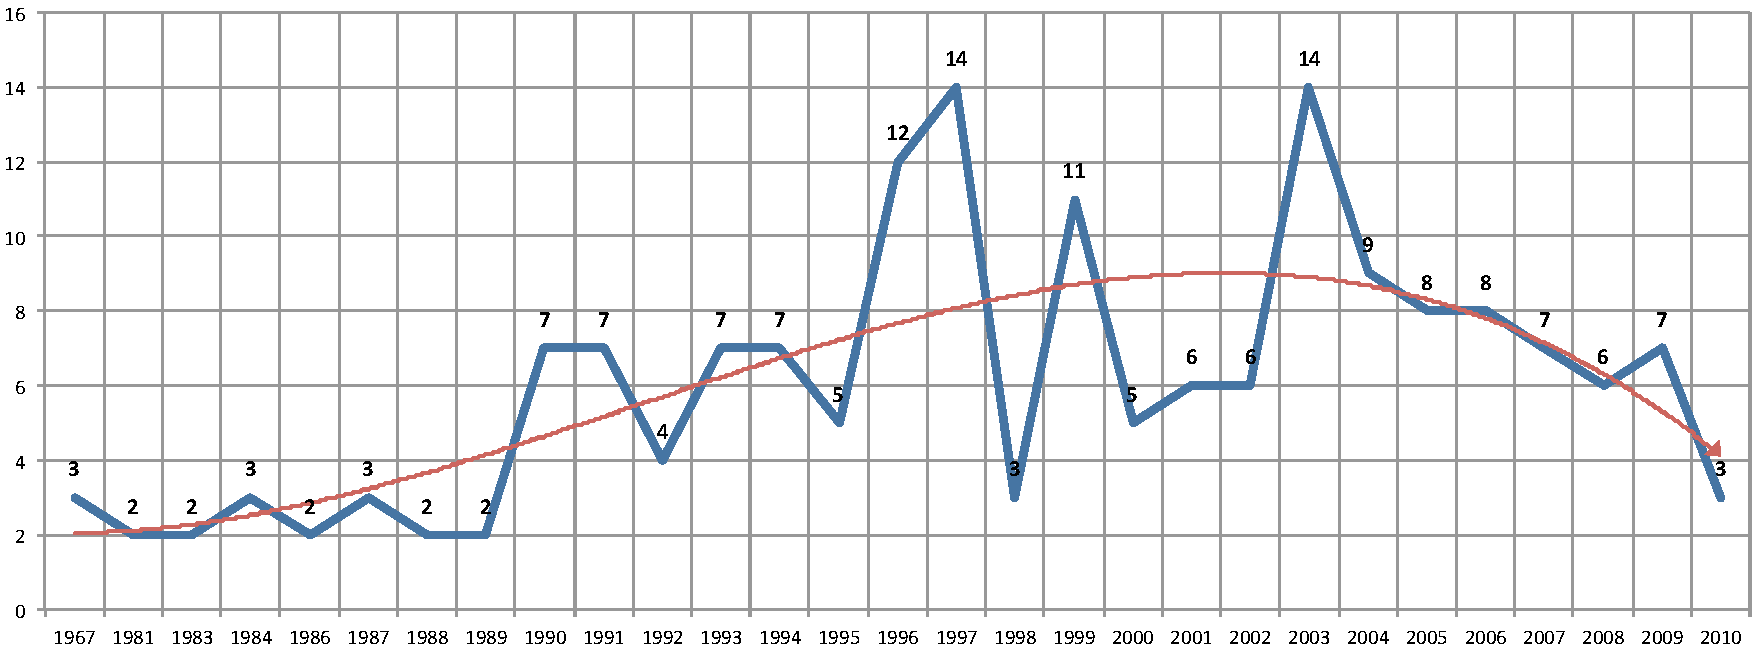
\includegraphics[scale=0.5]{abntex2-modelo-img-grafico.pdf}
	\end{center}
	\legend{Fonte: \citeonline[p. 24]{araujo2012}}
\end{figure}

% ---
\subsection{Figuras em \emph{minipages}}
% ---

\emph{Minipages} são usadas para inserir textos ou outros elementos em quadros
com tamanhos e posições controladas. Veja o exemplo da
\autoref{fig_minipage_imagem1} e da \autoref{fig_minipage_grafico2}.

\begin{figure}[htb]
 \label{teste}
 \centering
  \begin{minipage}{0.4\textwidth}
    \centering
    \caption{Imagem 1 da minipage} \label{fig_minipage_imagem1}
    
\includegraphics[scale=0.9]{abntex2-modelo-img-marca.pdf}
    \legend{Fonte: Produzido pelos autores}
  \end{minipage}
  \hfill
  \begin{minipage}{0.4\textwidth}
    \centering
    \caption{Grafico 2 da minipage} \label{fig_minipage_grafico2}
    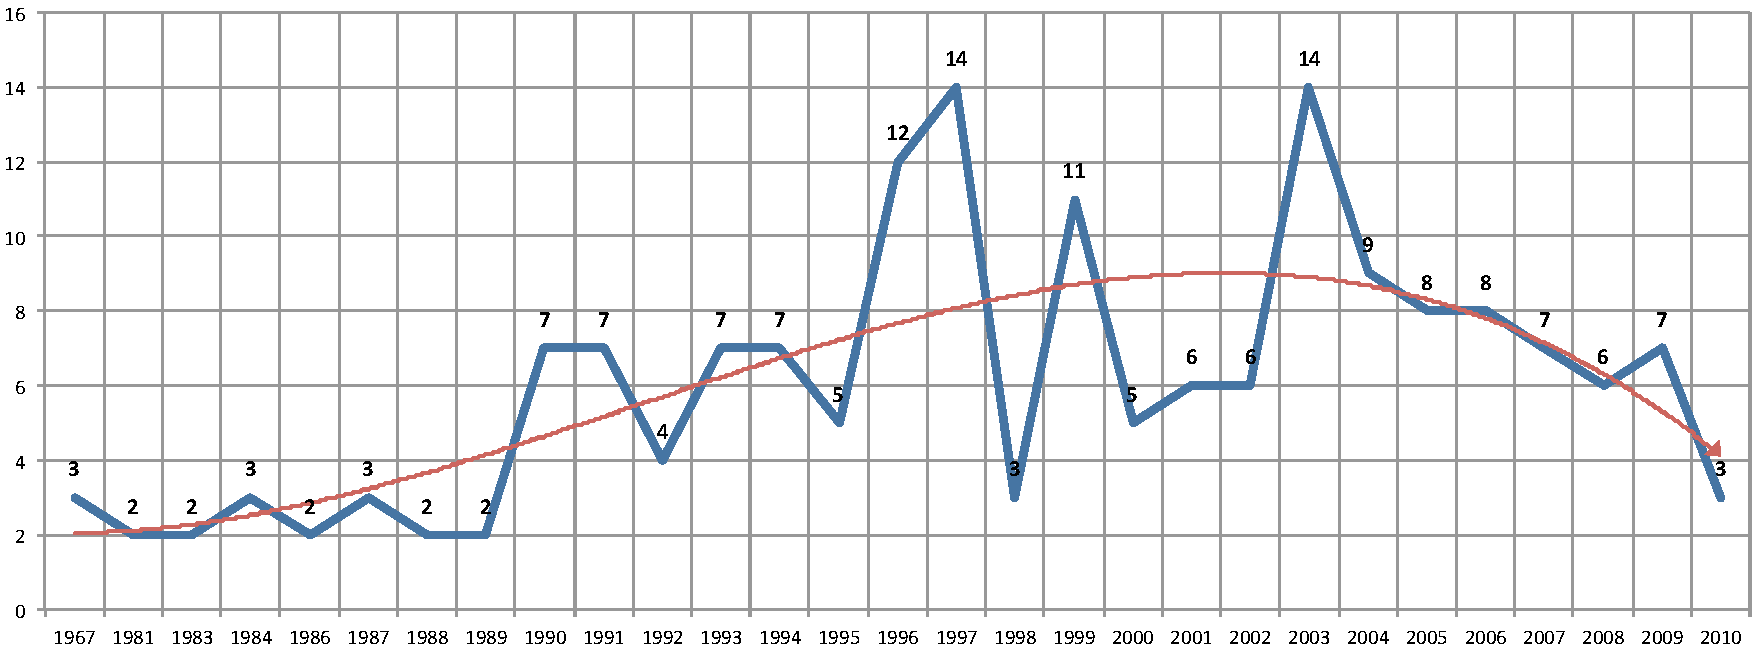
\includegraphics[scale=0.2]{abntex2-modelo-img-grafico.pdf}
    \legend{Fonte: \citeonline[p. 24]{araujo2012}}
  \end{minipage}
\end{figure}

Observe que, segundo a \citeonline[seções 4.2.1.10 e 5.8]{NBR14724:2011}, as
ilustrações devem sempre ter numeração contínua e única em todo o documento:

\begin{citacao}
Qualquer que seja o tipo de ilustração, sua identificação aparece na parte
superior, precedida da palavra designativa (desenho, esquema, fluxograma,
fotografia, gráfico, mapa, organograma, planta, quadro, retrato, figura,
imagem, entre outros), seguida de seu número de ordem de ocorrência no texto,
em algarismos arábicos, travessão e do respectivo título. Após a ilustração, na
parte inferior, indicar a fonte consultada (elemento obrigatório, mesmo que
seja produção do próprio autor), legenda, notas e outras informações
necessárias à sua compreensão (se houver). A ilustração deve ser citada no
texto e inserida o mais próximo possível do trecho a que se
refere. \cite[seções 5.8]{NBR14724:2011}
\end{citacao}

% ---
\section{Expressões matemáticas}
% ---

\index{expressões matemáticas}Use o ambiente \texttt{equation} para escrever
expressões matemáticas numeradas:

\begin{equation}
  \forall x \in X, \quad \exists \: y \leq \epsilon
\end{equation}

Escreva expressões matemáticas entre \$ e \$, como em $ \lim_{x \to \infty}
\exp(-x) = 0 $, para que fiquem na mesma linha.

Também é possível usar colchetes para indicar o início de uma expressão
matemática que não é numerada.

\[
\left|\sum_{i=1}^n a_ib_i\right|
\le
\left(\sum_{i=1}^n a_i^2\right)^{1/2}
\left(\sum_{i=1}^n b_i^2\right)^{1/2}
\]

Consulte mais informações sobre expressões matemáticas em
\url{https://code.google.com/p/abntex2/wiki/Referencias}.

% ---
\section{Enumerações: alíneas e subalíneas}
% ---

\index{alíneas}\index{subalíneas}\index{incisos}Quando for necessário enumerar
os diversos assuntos de uma seção que não possua título, esta deve ser
subdividida em alíneas \cite[4.2]{NBR6024:2012}:

\begin{alineas}

  \item os diversos assuntos que não possuam título próprio, dentro de uma mesma
  seção, devem ser subdivididos em alíneas; 
  
  \item o texto que antecede as alíneas termina em dois pontos;
  \item as alíneas devem ser indicadas alfabeticamente, em letra minúscula,
  seguida de parêntese. Utilizam-se letras dobradas, quando esgotadas as
  letras do alfabeto;

  \item as letras indicativas das alíneas devem apresentar recuo em relação à
  margem esquerda;

  \item o texto da alínea deve começar por letra minúscula e terminar em
  ponto-e-vírgula, exceto a última alínea que termina em ponto final;

  \item o texto da alínea deve terminar em dois pontos, se houver subalínea;

  \item a segunda e as seguintes linhas do texto da alínea começa sob a
  primeira letra do texto da própria alínea;
  
  \item subalíneas \cite[4.3]{NBR6024:2012} devem ser conforme as alíneas a
  seguir:

  \begin{alineas}
     \item as subalíneas devem começar por travessão seguido de espaço;

     \item as subalíneas devem apresentar recuo em relação à alínea;

     \item o texto da subalínea deve começar por letra minúscula e terminar em
     ponto-e-vírgula. A última subalínea deve terminar em ponto final, se não
     houver alínea subsequente;

     \item a segunda e as seguintes linhas do texto da subalínea começam sob a
     primeira letra do texto da própria subalínea.
  \end{alineas}
  
  \item no \abnTeX\ estão disponíveis os ambientes \texttt{incisos} e
  \texttt{subalineas}, que em suma são o mesmo que se criar outro nível de
  \texttt{alineas}, como nos exemplos à seguir:
  
  \begin{incisos}
    \item \textit{Um novo inciso em itálico};
  \end{incisos}
  
  \item Alínea em \textbf{negrito}:
  
  \begin{subalineas}
    \item \textit{Uma subalínea em itálico};
    \item \underline{\textit{Uma subalínea em itálico e sublinhado}}; 
  \end{subalineas}
  
  \item Última alínea com \emph{ênfase}.
  
\end{alineas}

% ---
\section{Espaçamento entre parágrafos e linhas}
% ---

\index{espaçamento!dos parágrafos}O tamanho do parágrafo, espaço entre a margem
e o início da frase do parágrafo, é definido por:

\begin{verbatim}
   \setlength{\parindent}{1.3cm}
\end{verbatim}

\index{espaçamento!do primeiro parágrafo}Por padrão, não há espaçamento no
primeiro parágrafo de cada início de divisão do documento
(\autoref{sec-divisoes}). Porém, você pode definir que o primeiro parágrafo
também seja indentado, como é o caso deste documento. Para isso, apenas inclua o
pacote \textsf{indentfirst} no preâmbulo do documento:

\begin{verbatim}
   \usepackage{indentfirst}      % Indenta o primeiro parágrafo de cada seção.
\end{verbatim}

\index{espaçamento!entre os parágrafos}O espaçamento entre um parágrafo e outro
pode ser controlado por meio do comando:

\begin{verbatim}
  \setlength{\parskip}{0.2cm}  % tente também \onelineskip
\end{verbatim}

\index{espaçamento!entre as linhas}O controle do espaçamento entre linhas é
definido por:

\begin{verbatim}
  \OnehalfSpacing       % espaçamento um e meio (padrão); 
  \DoubleSpacing        % espaçamento duplo
  \SingleSpacing        % espaçamento simples	
\end{verbatim}

Para isso, também estão disponíveis os ambientes:

\begin{verbatim}
  \begin{SingleSpace} ...\end{SingleSpace}
  \begin{Spacing}{hfactori} ... \end{Spacing}
  \begin{OnehalfSpace} ... \end{OnehalfSpace}
  \begin{OnehalfSpace*} ... \end{OnehalfSpace*}
  \begin{DoubleSpace} ... \end{DoubleSpace}
  \begin{DoubleSpace*} ... \end{DoubleSpace*} 
\end{verbatim}

Para mais informações, consulte \citeonline[p. 47-52 e 135]{memoir}.

% ---
\section{Inclusão de outros arquivos}\label{sec-include}
% ---

É uma boa prática dividir o seu documento em diversos arquivos, e não
apenas escrever tudo em um único. Esse recurso foi utilizado neste
documento. Para incluir diferentes arquivos em um arquivo principal,
de modo que cada arquivo incluído fique em uma página diferente, utilize o
comando:

\begin{verbatim}
   \include{documento-a-ser-incluido}      % sem a extensão .tex
\end{verbatim}

Para incluir documentos sem quebra de páginas, utilize:

\begin{verbatim}
   \input{documento-a-ser-incluido}      % sem a extensão .tex
\end{verbatim}

% ---
\section{Compilar o documento \LaTeX}
% ---

Geralmente os editores \LaTeX, como o
TeXlipse\footnote{\url{http://texlipse.sourceforge.net/}}, o
Texmaker\footnote{\url{http://www.xm1math.net/texmaker/}}, entre outros,
compilam os documentos automaticamente, de modo que você não precisa se
preocupar com isso.

No entanto, você pode compilar os documentos \LaTeX usando os seguintes
comandos, que devem ser digitados no \emph{Prompt de Comandos} do Windows ou no
\emph{Terminal} do Mac ou do Linux:

\begin{verbatim}
   pdflatex ARQUIVO_PRINCIPAL.tex
   bibtex ARQUIVO_PRINCIPAL.aux
   makeindex ARQUIVO_PRINCIPAL.idx 
   makeindex ARQUIVO_PRINCIPAL.nlo -s nomencl.ist -o ARQUIVO_PRINCIPAL.nls
   pdflatex ARQUIVO_PRINCIPAL.tex
   pdflatex ARQUIVO_PRINCIPAL.tex
\end{verbatim}

% ---
\section{Remissões internas}
% ---

Ao nomear a \autoref{tab-nivinv} e a \autoref{fig_circulo}, apresentamos um
exemplo de remissão interna, que também pode ser feita quando indicamos o
\autoref{cap_exemplos}, que tem o nome \emph{\nameref{cap_exemplos}}. O número
do capítulo indicado é \ref{cap_exemplos}, que se inicia à
\autopageref{cap_exemplos}\footnote{O número da página de uma remissão pode ser
obtida também assim:
\pageref{cap_exemplos}.}.
Veja a \autoref{sec-divisoes} para outros exemplos de remissões internas entre
seções, subseções e subsubseções.

O código usado para produzir o texto desta seção é:

\begin{verbatim}
Ao nomear a \autoref{tab-nivinv} e a \autoref{fig_circulo}, apresentamos um
exemplo de remissão interna, que também pode ser feita quando indicamos o
\autoref{cap_exemplos}, que tem o nome \emph{\nameref{cap_exemplos}}. O número
do capítulo indicado é \ref{cap_exemplos}, que se inicia à
\autopageref{cap_exemplos}\footnote{O número da página de uma remissão pode ser
obtida também assim:
\pageref{cap_exemplos}.}.
Veja a \autoref{sec-divisoes} para outros exemplos de remissões internas entre
seções, subseções e subsubseções.
\end{verbatim}

% ---
\section{Divisões do documento: seção}\label{sec-divisoes}
% ---

Esta seção testa o uso de divisões de documentos. Esta é a
\autoref{sec-divisoes}. Veja a \autoref{sec-divisoes-subsection}.

\subsection{Divisões do documento: subseção}\label{sec-divisoes-subsection}

Isto é uma subseção. Veja a \autoref{sec-divisoes-subsubsection}, que é uma
\texttt{subsubsection} do \LaTeX, mas é impressa chamada de ``subseção'' porque
no Português não temos a palavra ``subsubseção''.

\subsubsection{Divisões do documento: subsubseção}
\label{sec-divisoes-subsubsection}

Isto é uma subsubseção.

\subsubsection{Divisões do documento: subsubseção}

Isto é outra subsubseção.

\subsection{Divisões do documento: subseção}\label{sec-exemplo-subsec}

Isto é uma subseção.

\subsubsection{Divisões do documento: subsubseção}

Isto é mais uma subsubseção da \autoref{sec-exemplo-subsec}.


\subsubsubsection{Esta é uma subseção de quinto
nível}\label{sec-exemplo-subsubsubsection}

Esta é uma seção de quinto nível. Ela é produzida com o seguinte comando:

\begin{verbatim}
\subsubsubsection{Esta é uma subseção de quinto
nível}\label{sec-exemplo-subsubsubsection}
\end{verbatim}

\subsubsubsection{Esta é outra subseção de quinto nível}\label{sec-exemplo-subsubsubsection-outro}

Esta é outra seção de quinto nível.


\paragraph{Este é um parágrafo numerado}\label{sec-exemplo-paragrafo}

Este é um exemplo de parágrafo nomeado. Ele é produzida com o comando de
parágrafo:

\begin{verbatim}
\paragraph{Este é um parágrafo nomeado}\label{sec-exemplo-paragrafo}
\end{verbatim}

A numeração entre parágrafos numeradaos e subsubsubseções são contínuas.

\paragraph{Esta é outro parágrafo numerado}\label{sec-exemplo-paragrafo-outro}

Esta é outro parágrafo nomeado.

% ---
\section{Este é um exemplo de nome de seção longo. Ele deve estar
alinhado à esquerda e a segunda e demais linhas devem iniciar logo abaixo da
primeira palavra da primeira linha}
% ---

Isso atende à norma \citeonline[seções de 5.2.2 a 5.2.4]{NBR14724:2011} 
 e \citeonline[seções de 3.1 a 3.8]{NBR6024:2012}.

% ---
\section{Diferentes idiomas e hifenizações}
\label{sec-hifenizacao}
% ---

Para usar hifenizações de diferentes idiomas, inclua nas opções do documento o
nome dos idiomas que o seu texto contém. Por exemplo (para melhor
visualização, as opções foram quebras em diferentes linhas):

\begin{verbatim}
\documentclass[
	12pt,
	openright,
	twoside,
	a4paper,
	english,
	french,
	spanish,
	brazil
	]{abntex2}
\end{verbatim}

O idioma português-brasileiro (\texttt{brazil}) é incluído automaticamente pela
classe \textsf{abntex2}. Porém, mesmo assim a opção \texttt{brazil} deve ser
informada como a última opção da classe para que todos os pacotes reconheçam o
idioma. Vale ressaltar que a última opção de idioma é a utilizada por padrão no
documento. Desse modo, caso deseje escrever um texto em inglês que tenha
citações em português e em francês, você deveria usar o preâmbulo como abaixo:

\begin{verbatim}
\documentclass[
	12pt,
	openright,
	twoside,
	a4paper,
	french,
	brazil,
	english
	]{abntex2}
\end{verbatim}

A lista completa de idiomas suportados, bem como outras opções de hifenização,
estão disponíveis em \citeonline[p.~5-6]{babel}.

Exemplo de hifenização em inglês\footnote{Extraído de:
\url{http://en.wikibooks.org/wiki/LaTeX/Internationalization}}:

\begin{otherlanguage*}{english}
\textit{Text in English language. This environment switches all language-related
definitions, like the language specific names for figures, tables etc. to the other
language. The starred version of this environment typesets the main text
according to the rules of the other language, but keeps the language specific
string for ancillary things like figures, in the main language of the document.
The environment hyphenrules switches only the hyphenation patterns used; it can
also be used to disallow hyphenation by using the language name
`nohyphenation'.}
\end{otherlanguage*}

Exemplo de hifenização em francês\footnote{Extraído de:
\url{http://bigbrowser.blog.lemonde.fr/2013/02/17/tu-ne-tweeteras-point-le-vatican-interdit-aux-cardinaux-de-tweeter-pendant-le-conclave/}}:

\begin{otherlanguage*}{french}
\textit{Texte en français. Pas question que Twitter ne vienne faire une
concurrence déloyale à la traditionnelle fumée blanche qui marque l'élection
d'un nouveau pape. Pour éviter toute fuite précoce, le Vatican a donc pris un
peu d'avance, et a déjà interdit aux cardinaux qui prendront part au vote
d'utiliser le réseau social, selon Catholic News Service. Une mesure valable
surtout pour les neuf cardinaux – sur les 117 du conclave – pratiquants très
actifs de Twitter, qui auront interdiction pendant toute la période de se
connecter à leur compte.}
\end{otherlanguage*}

Pequeno texto em espanhol\footnote{Extraído de:
\url{http://internacional.elpais.com/internacional/2013/02/17/actualidad/1361102009_913423.html}}:

\foreignlanguage{spanish}{\textit{Decenas de miles de personas ovacionan al pontífice en su
penúltimo ángelus dominical, el primero desde que anunciase su renuncia. El Papa se
centra en la crítica al materialismo}}.

O idioma geral do texto por ser alterado como no exemplo seguinte:

\begin{verbatim}
  \selectlanguage{english}
\end{verbatim}

Isso altera automaticamente a hifenização e todos os nomes constantes de
referências do documento para o idioma inglês. Consulte o manual da classe
\cite{abntex2classe} para obter orientações adicionais sobre internacionalização de
documentos produzidos com \abnTeX.

A \autoref{sec-citacao} descreve o ambiente \texttt{citacao} que pode receber
como parâmetro um idioma a ser usado na citação.

% ---
\section{Consulte o manual da classe \textsf{abntex2}}
% ---

Consulte o manual da classe \textsf{abntex2} \cite{abntex2classe} para uma
referência completa das macros e ambientes disponíveis. 

Além disso, o manual possui informações adicionais sobre as normas ABNT
observadas pelo \abnTeX\ e considerações sobre eventuais requisitos específicos
não atendidos, como o caso da \citeonline[seção 5.2.2]{NBR14724:2011}, que
especifica o espaçamento entre os capítulos e o início do texto, regra
propositalmente não atendida pelo presente modelo.

% ---
\section{Referências bibliográficas}
% ---

A formatação das referências bibliográficas conforme as regras da ABNT são um
dos principais objetivos do \abnTeX. Consulte os manuais
\citeonline{abntex2cite} e \citeonline{abntex2cite-alf} para obter informações
sobre como utilizar as referências bibliográficas.

%-
\subsection{Acentuação de referências bibliográficas}
%-

Normalmente não há problemas em usar caracteres acentuados em arquivos
bibliográficos (\texttt{*.bib}). Porém, como as regras da ABNT fazem uso quase
abusivo da conversão para letras maiúsculas, é preciso observar o modo como se
escreve os nomes dos autores. Na ~\autoref{tabela-acentos} você encontra alguns
exemplos das conversões mais importantes. Preste atenção especial para `ç' e `í'
que devem estar envoltos em chaves. A regra geral é sempre usar a acentuação
neste modo quando houver conversão para letras maiúsculas.

\begin{table}[htbp]
\caption{Tabela de conversão de acentuação.}
\label{tabela-acentos}

\begin{center}
\begin{tabular}{ll}\hline\hline
acento & \textsf{bibtex}\\
à á ã & \verb+\`a+ \verb+\'a+ \verb+\~a+\\
í & \verb+{\'\i}+\\
ç & \verb+{\c c}+\\
\hline\hline
\end{tabular}
\end{center}
\end{table}


% ---
\section{Precisa de ajuda?}
% ---

Consulte a FAQ com perguntas frequentes e comuns no portal do \abnTeX:
\url{https://code.google.com/p/abntex2/wiki/FAQ}.

Inscreva-se no grupo de usuários \LaTeX:
\url{http://groups.google.com/group/latex-br}, tire suas dúvidas e ajude
outros usuários.

Participe também do grupo de desenvolvedores do \abnTeX:
\url{http://groups.google.com/group/abntex2} e faça sua contribuição à
ferramenta.

% ---
\section{Você pode ajudar?}
% ---

Sua contribuição é muito importante! Você pode ajudar na divulgação, no
desenvolvimento e de várias outras formas. Veja como contribuir com o \abnTeX\
em \url{https://code.google.com/p/abntex2/wiki/ComoContribuir}.

% ---
\section{Quer customizar os modelos do \abnTeX\ para sua instituição ou
universidade?}
% ---

Veja como customizar o \abnTeX\ em:
\url{https://code.google.com/p/abntex2/wiki/ComoCustomizar}.


% ---

% ----------------------------------------------------------
% PARTE
% ----------------------------------------------------------
%\part{Referenciais teóricos}
% ----------------------------------------------------------

% ---
% Capitulo de revisão de literatura
% ---
\chapter{Apresentação da Empresa}

A RBS TV é uma emissora de televisão afiliada da Rede Globo, com atuação nos estados do Rio Grande do Sul e Santa Catarina, na região sul do Brasil. Além de retransmitir a programação da Rede Globo na maior parte do tempo, também exibe produções próprias diariamente, nos segmentos informativos e de entretenimento.

Para garantir a ampliação e a manutenção de sua infraestrutura, a empresa tem uma grande equipe técnica que atua projetando a implantação de novas tecnologias e prestando suporte à infraestrutura existente. A equipe técnica é composta de engenheiros e técnicos em eletrônica

\section{GPAC}
\section{The FFmpeg framework}

\begin{figure}[!h]
\centering
\caption{Pointer assignment example.}
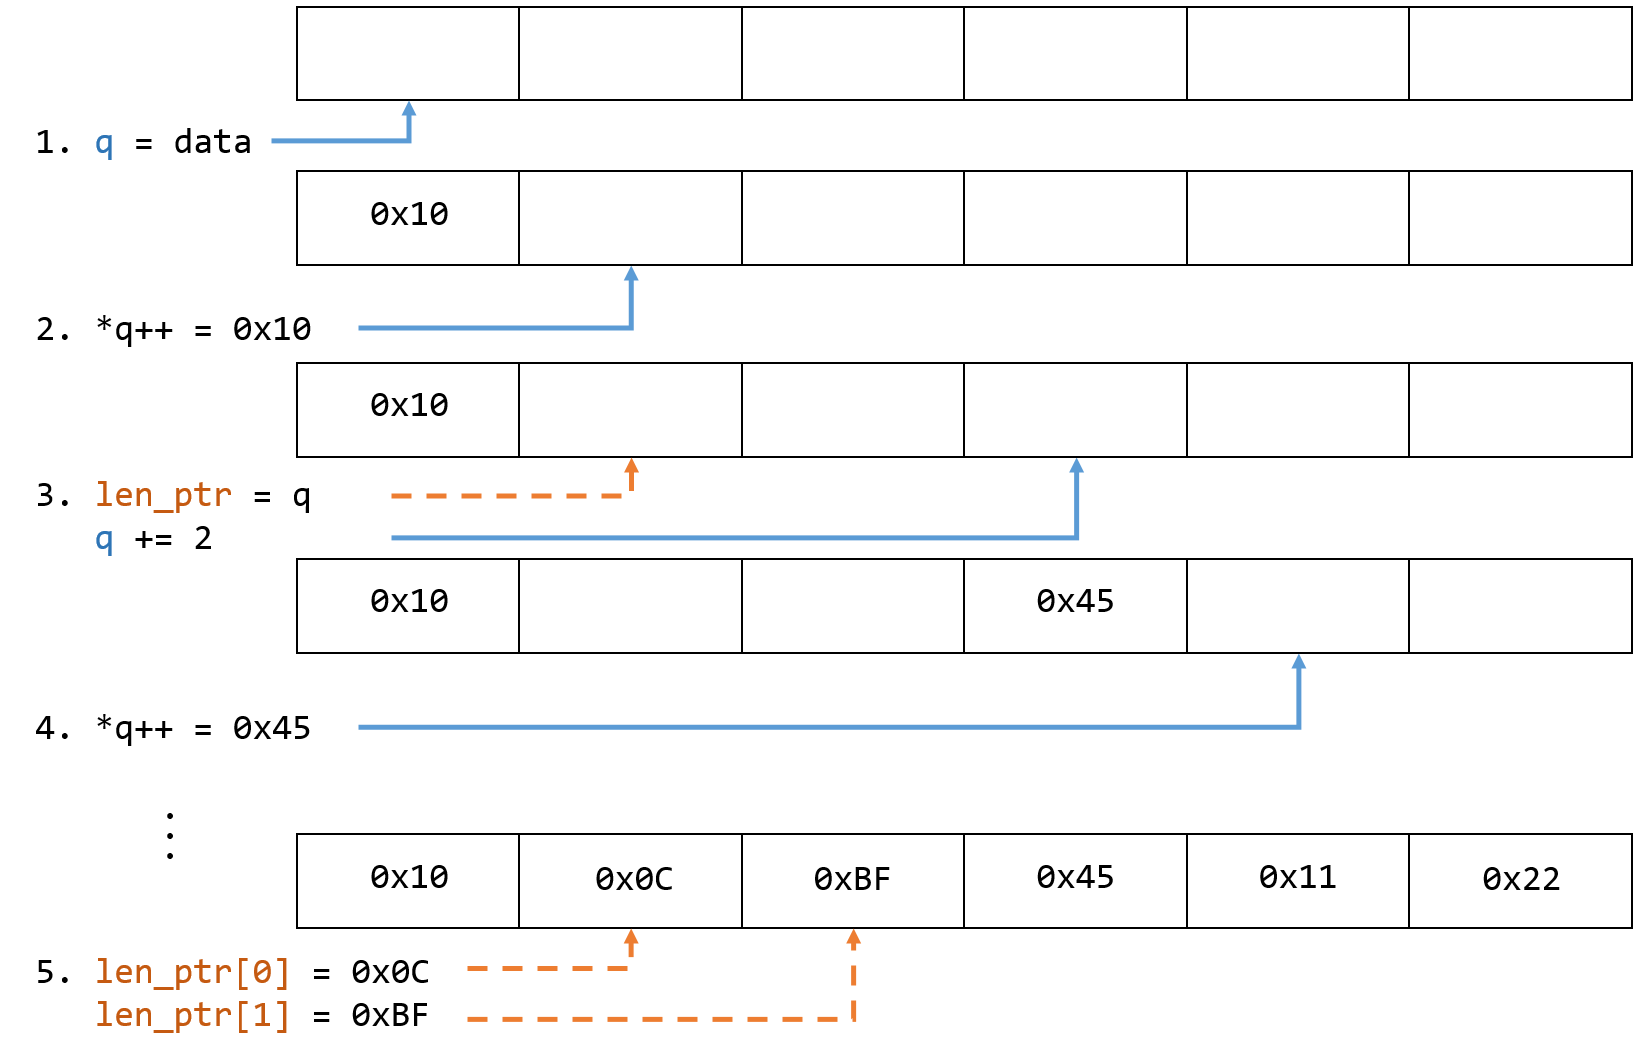
\includegraphics[width=0.8\linewidth]{figuras/pointer_assignment.png}
\\Source: The author.
\label{fig:pointer_assignment}
\end{figure}

\subsection{Descriptors}
% ---
% Conclusão (outro exemplo de capítulo sem numeração e presente no sumário)
% ---
\chapter[Conclusões]{Conclusões}
%\addcontentsline{toc}{chapter}{Conclusions and Future Development}
% ---

% ----------------------------------------------------------
% ELEMENTOS PÓS-TEXTUAIS
% ----------------------------------------------------------
\postextual
% ----------------------------------------------------------

% ----------------------------------------------------------
% Referências bibliográficas
% ----------------------------------------------------------
\bibliography{relatorio_estagio}

% ----------------------------------------------------------
% Glossário
% ----------------------------------------------------------
%
% Consulte o manual da classe abntex2 para orientações sobre o glossário.
%
%\glossary

% ----------------------------------------------------------
% Apêndices
% ----------------------------------------------------------

% ---
% Inicia os apêndices
% ---
\begin{apendicesenv}

% Imprime uma página indicando o início dos apêndices, Documento ou texto elaborado pelo autor
\partapendices

\chapter{Modulation aspects of the SBTVD Standard}
\label{modulation}
% ---
In ISDB-T, a UHF channel is split into 13 frequency segments. The narrow-band receivers, which are capable of decoding only the central channel frequency(or segment), is commonly called a 1-segment receiver. The wide-band receivers, that can decode all the 13 frequency segments, are called full-segment decoders. \autoref{fig:ISDB-T_CH_Seg_Prog_allocation} shows the segment distribution inside a channel. 'S0' is the central segment for narrow-band tuners. 'S1' to 'S12' are the other segments. As narrower the band, as smaller is the amount of information that can be sent through it. 1-Segment receivers are used in mobile devices, and are capable of receive low definition video only, along with one single audio stream. Full-segment receivers are used in fixed devices, such as Full-HD TVs, and are capable of decode high definition video along with multiple audio streams.

The modulation schemes usually used in 'S0' are different than the ones of the other segments. Since 1-segment TV is targeted for mobile devices, the signal reach should be higher and at most a small dipole antenna is availlable, then QPSK modulation is used. For the other segments, the amount of data is much higher, and customers don't mind to have an amplified antenna attached to the back of their TV, so less robust modulation is applied, such as 64QAM. 

\begin{figure}
\centering
\caption{ISDB-T channel, segment and program allocation.}
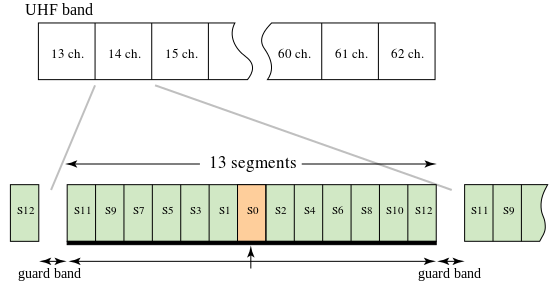
\includegraphics[width=0.8\linewidth]{figuras/ISDB-T_CH_Seg_Prog_allocation.png}
\\Source: .
\label{fig:ISDB-T_CH_Seg_Prog_allocation}
\end{figure}

% ----------------------------------------------------------
\end{apendicesenv}
% ---


% ----------------------------------------------------------
% Anexos
% ----------------------------------------------------------

% ---
% Inicia os anexos, Documento ou texto NÃO elaborado pelo autor
% ---
\begin{anexosenv}

% Imprime uma página indicando o início dos anexos
\partanexos

% ---

% ---
%\chapter{Cras non urna sed feugiat cum sociis natoque penatibus et magnis dis
%parturient montes nascetur ridiculus mus}
% ---

%\lipsum[31]

% ---
\end{anexosenv}

%---------------------------------------------------------------------
% INDICE REMISSIVO
%---------------------------------------------------------------------
\phantompart
\printindex
%---------------------------------------------------------------------

\end{document}
